
\begin{figure}
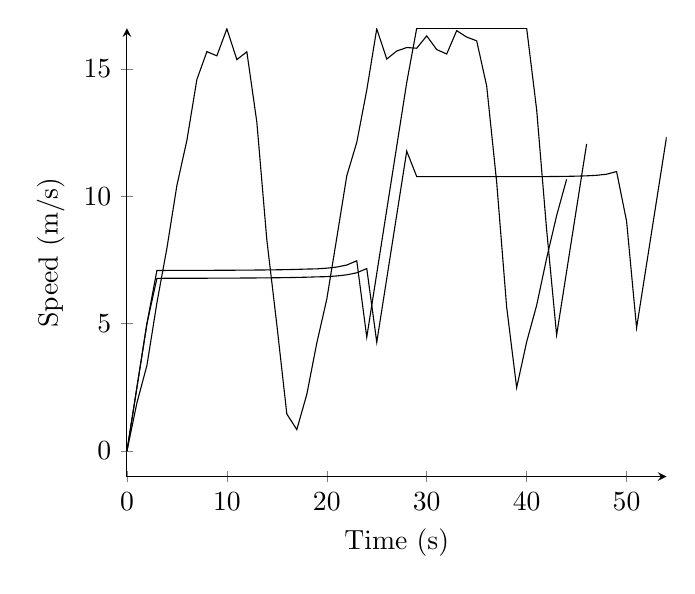
\begin{tikzpicture}
\begin{axis}[
legend style={
	anchor=west
},
axis x line=bottom,
axis y line=left,
ymin=-1,
point meta=explicit symbolic,
xlabel=Time (s),
ylabel=Speed (m/s)
]
\addplot[] coordinates {
(0, 0.0)
(1, 1.89374451642)
(2, 3.36139972205)
(3, 5.81963361037)
(4, 7.96200727782)
(5, 10.4275545923)
(6, 12.1972315881)
(7, 14.5870819522)
(8, 15.6803324539)
(9, 15.5166591925)
(10, 16.576352134)
(11, 15.3687371683)
(12, 15.6738290321)
(13, 12.9134948644)
(14, 8.28956257431)
(15, 4.96313414158)
(16, 1.45690722736)
(17, 0.843999729409)
(18, 2.22809304207)
(19, 4.24151234577)
(20, 5.96348795909)
(21, 8.37138129501)
(22, 10.806048799)
(23, 12.1195751928)
(24, 14.1714825503)
(25, 16.5754516967)
(26, 15.3909995159)
(27, 15.7045815943)
(28, 15.8420380175)
(29, 15.8148368122)
(30, 16.300192376)
(31, 15.7613223488)
(32, 15.5873101117)
(33, 16.505332613)
(34, 16.2511732665)
(35, 16.1053755844)
(36, 14.3320566202)
(37, 10.5583155233)
(38, 5.64755013615)
(39, 2.49245426008)
(40, 4.28636383237)
(41, 5.72162774189)
(42, 7.56817731396)
(43, 9.24669719506)
(44, 10.6685672072)
};
\addplot[] coordinates {
(0, 0.0)
(1, 2.5)
(2, 5.0)
(3, 6.7820275515)
(4, 6.78271748663)
(5, 6.78350051155)
(6, 6.78439418679)
(7, 6.78542042564)
(8, 6.78660685887)
(9, 6.7879887272)
(10, 6.7896115492)
(11, 6.7915349511)
(12, 6.79383827713)
(13, 6.79662899748)
(14, 6.80005563744)
(15, 6.80432825212)
(16, 6.80975196909)
(17, 6.81678416163)
(18, 6.8261365924)
(19, 6.83896857447)
(20, 6.84730669373)
(21, 6.87485714822)
(22, 6.91921659518)
(23, 6.99835841228)
(24, 7.16583078852)
(25, 4.27276145066)
(26, 6.77276145066)
(27, 9.27276145066)
(28, 11.7727614507)
(29, 10.7748110565)
(30, 10.7748389045)
(31, 10.7748709099)
(32, 10.7749079434)
(33, 10.7749511168)
(34, 10.7750018666)
(35, 10.7750620761)
(36, 10.7751342523)
(37, 10.775221792)
(38, 10.7753293892)
(39, 10.7754636795)
(40, 10.7756342906)
(41, 10.7758556221)
(42, 10.7759963436)
(43, 10.7796551597)
(44, 10.7848625152)
(45, 10.7926366216)
(46, 10.8049983634)
(47, 10.8264493688)
(48, 10.8688302741)
(49, 10.9727599752)
(50, 9.02390827769)
(51, 4.83655483095)
(52, 7.33655483095)
(53, 9.83655483095)
(54, 12.3365548309)
};
\addplot[] coordinates {
(0, 0.0)
(1, 2.5)
(2, 5.0)
(3, 7.09028751929)
(4, 7.09104453409)
(5, 7.09190891586)
(6, 7.09290200653)
(7, 7.09405073724)
(8, 7.09538948544)
(9, 7.09696269561)
(10, 7.0988286459)
(11, 7.10106497327)
(12, 7.10377696545)
(13, 7.10711033187)
(14, 7.111271463)
(15, 7.11656068412)
(16, 7.12342905814)
(17, 7.1325801111)
(18, 7.1451627221)
(19, 7.15317293179)
(20, 7.1803443926)
(21, 7.2242693585)
(22, 7.30304397506)
(23, 7.47090594595)
(24, 4.47049141946)
(25, 6.97049141946)
(26, 9.47049141946)
(27, 11.9704914195)
(28, 14.4704914195)
(29, 16.6)
(30, 16.6)
(31, 16.6)
(32, 16.6)
(33, 16.6)
(34, 16.6)
(35, 16.6)
(36, 16.6)
(37, 16.6)
(38, 16.6)
(39, 16.6)
(40, 16.6)
(41, 13.4031364835)
(42, 8.68482439784)
(43, 4.55585973861)
(44, 7.05585973861)
(45, 9.55585973861)
(46, 12.0558597386)
};

\end{axis}
\end{tikzpicture}
\label{tik:50:2_O, 2_O.-60, 4_S, 5_S, 5_S.-30, 6_V}
\caption{50 percent diving with GSC on route $2_O, 2_O.-60, 4_S, 5_S, 5_S.-30, 6_V$}
\end{figure}
